In this section we provide an overview of PaaS clouds and Cerebro. Then we present a model for 
negotiating response time SLAs for web APIs deployed in PaaS clouds.

PaaS clouds enforce a restricted programming model on the application developer to guarantee
the scalability, security and the availability of the cloud-hosted applications. To begin with,
PaaS clouds provide a predefined set of programming interfaces through which they export 
various platform services. We shall refer to these programming interfaces as the cloud software
development kit (cloud SDK). The cloud SDK exposes scalable functionality that can be used to 
program a wide range of application features. These include key-value data stores, databases, 
caching, task scheduling, and user management. In a typical PaaS environment
such as Google App Engine (or AppScale), the developer must use the cloud SDK to implement
all the required application components and APIs, as the use of third party services or libraries is
restricted within the cloud platform. 

Similarly, PaaS clouds may impose restrictions on performing
certain types of I/O operations, and executing long running tasks. For example, Google App Engine
does not allow applications to access the local file system, and all request processing threads must
terminate under 60 seconds. The result of all these restrictions is a programming model that is
amenable to reasoning via static analysis; a feature we exploit in the design of Cerebro. By surveying
a collection of open source PaaS applications we have also found that program features that typically
inhibit static analysis (e.g. excessive branching and loops) are scarce among PaaS-hosted
applications.

\begin{figure}
\centering
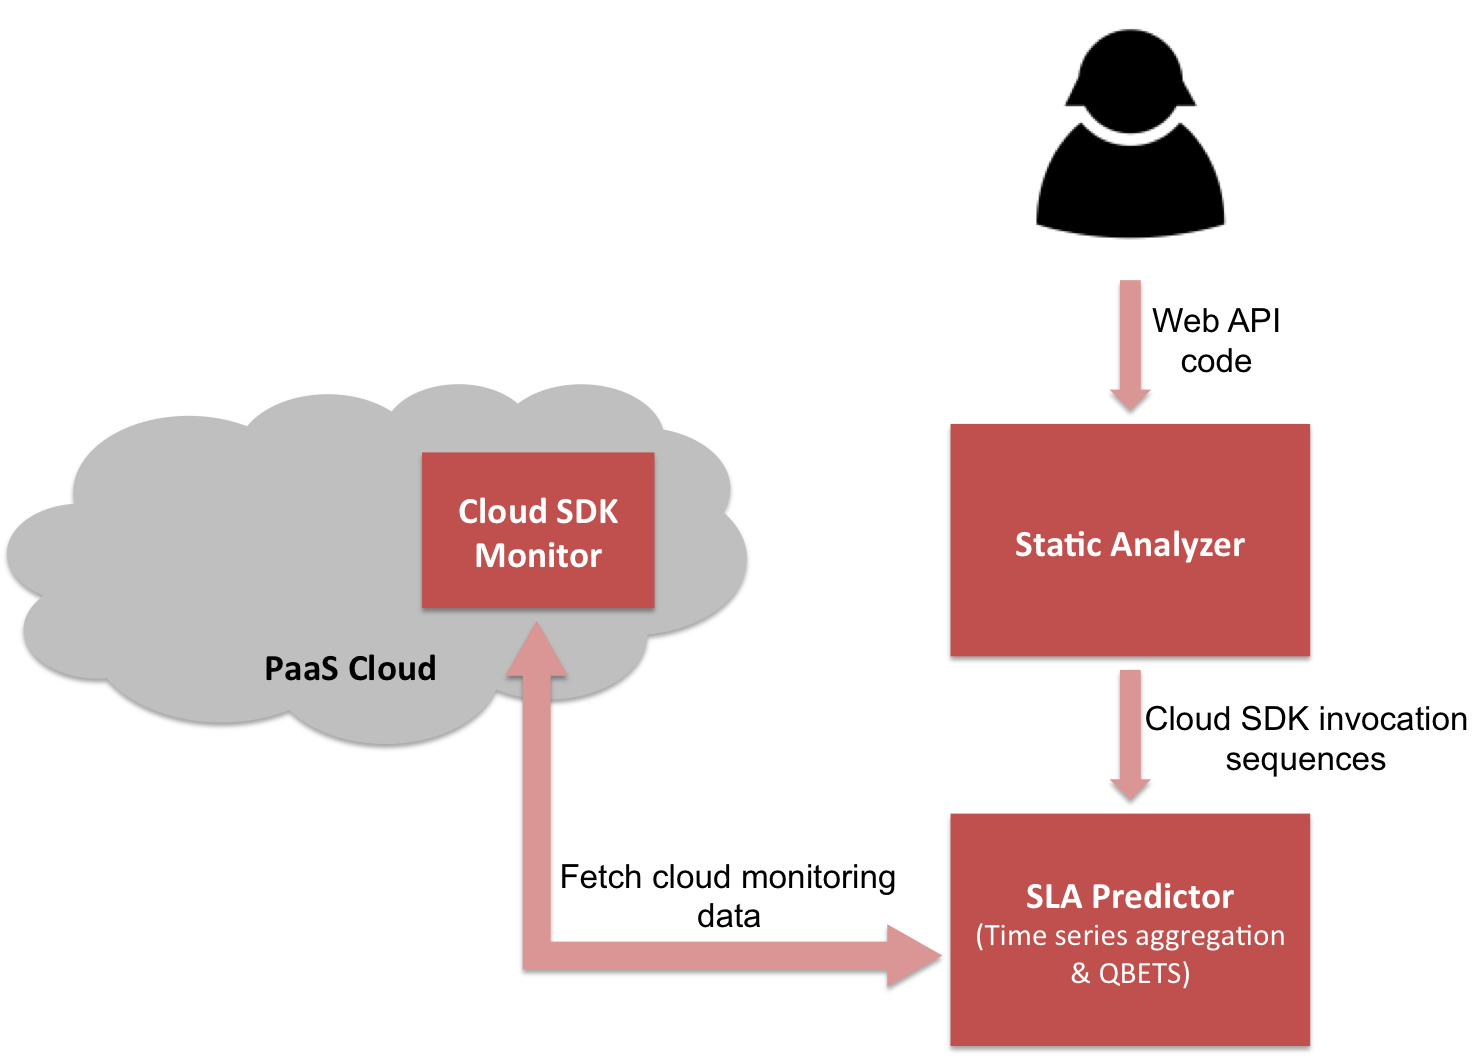
\includegraphics[scale=0.35]{cerebro_arch}
\caption{Main components of Cerebro and their interactions.}
\label{fig:cerebro_arch}
\vspace{-0.2in}
\end{figure}